%
% latex-sample.tex
%
% This LaTeX source file provides a template for a typical research paper.
%

%
% Use the standard article template.
%
\documentclass{article}

% The geometry package allows for easy page formatting.
\usepackage{geometry}
\geometry{letterpaper}
\usepackage{textcomp}
% Load up special logo commands.
\usepackage{doc}

% make a reference to Hypertext 
\usepackage{hyperref}

% Package for formatting URLs.
\usepackage{url}

% Packages and definitions for graphics files.
\usepackage{graphicx}
\usepackage{epstopdf}
%\DeclareGraphicsRule{.tif}{png}{.png}{`convert #1 'dirname #1'/'basename #1 .tif'.png}

%
% Set the title, author, and date.
%
\title{Economic Growth and Forest Area  \\ \small{DNSC 6211: Programming for Analytics}}
\author{
	Wei Zheng \\
}
\date{}

%
% The document proper.
%
\begin{document}

% Add the title section.
\maketitle

% Add an abstract.
\abstract{
For this project, I intend to investigate negative impacts of economic growth on forest areas at the national level. Using GDP and Forest Area data, I am able to look at trends of economic growth and forest area changes. To further assist my study, I group countries by their income levels.  And I calculate a Deforestation-GDP statistic and use ggplot to identify best and worst countries in each group. Hopefully, worst countries can draw lessons from best countries to protect their forests while improving their economies. Furthermore, to query about which continents have biggest deforestation problems, I create a world heat map. We can clearly see Latin America, Africa, and South Asia fare worst in term of deforestation. Finally, I run a linear regression to project forest areas of the worst country for the next two years using World Bank\textquotesingle s projected GDP data. It intends to answer the question what will happen if we do not reverse the trend for the nation.  


}

% Add various lists on new pages.
\pagebreak
\tableofcontents


% Start the paper on a new page.
\pagebreak

%
% Body text.
%
\section{Introduction}
\label{introduction}
This analysis focuses on the relationship between economic growth and deforestation. Economic growth is essential to improve people\textquotesingle s standard of living. On the other hand, forests play a very important role in protecting our environment. They absorb greenhouse gases and provide habitat for for millions of species.  Some countries are sacrificing their forests in order to grow their economies. This project tries to identify the best and worst countries at different income levels in term of forest area changes with respect to GDP growth. The worst countries can draw some lessons from the best countries to grow their economies without having grieving impacts on their forests. In addition, this project tries to identify the worst continents in term of deforestation.  Furthermore, the project also tries to project the forest area of the worst country in the world in term of deforestation for next two years given its projected GDP data. 

\section{Background}

In order to perform this analysis to answer guiding questions, I explored the World Bank’s datasets.  I was looking at Environment and Economy and Growth sections. Missing-value is a big issue for many datasets.  Finally, I chose Forest area and GDP, which are two relatively clean datasets. In order to group countries by income levels, I also download the countries’ meta data, which do not have API available. So I downloaded a csv instead.  I wanted to show negative impacts of deforestation on species. But the Mammal species(threatened) dataset has lots of missing values to be useful. So I gave up on the idea. 
\pagebreak
\section{Method}
I am able to create groups by income level. In those subgroups, I further investigate the relationship between GDP and Forest Areas. We clearly see high-income countries are better in protecting their forests than lower-income countries. But the datasets I have cannot explain why. I would like to further investigate the topic when relevant datasets become available. 

\subsection{Workflow}
The following diagram shows the project workflow.
\begin{figure}[hb]
  \centering
    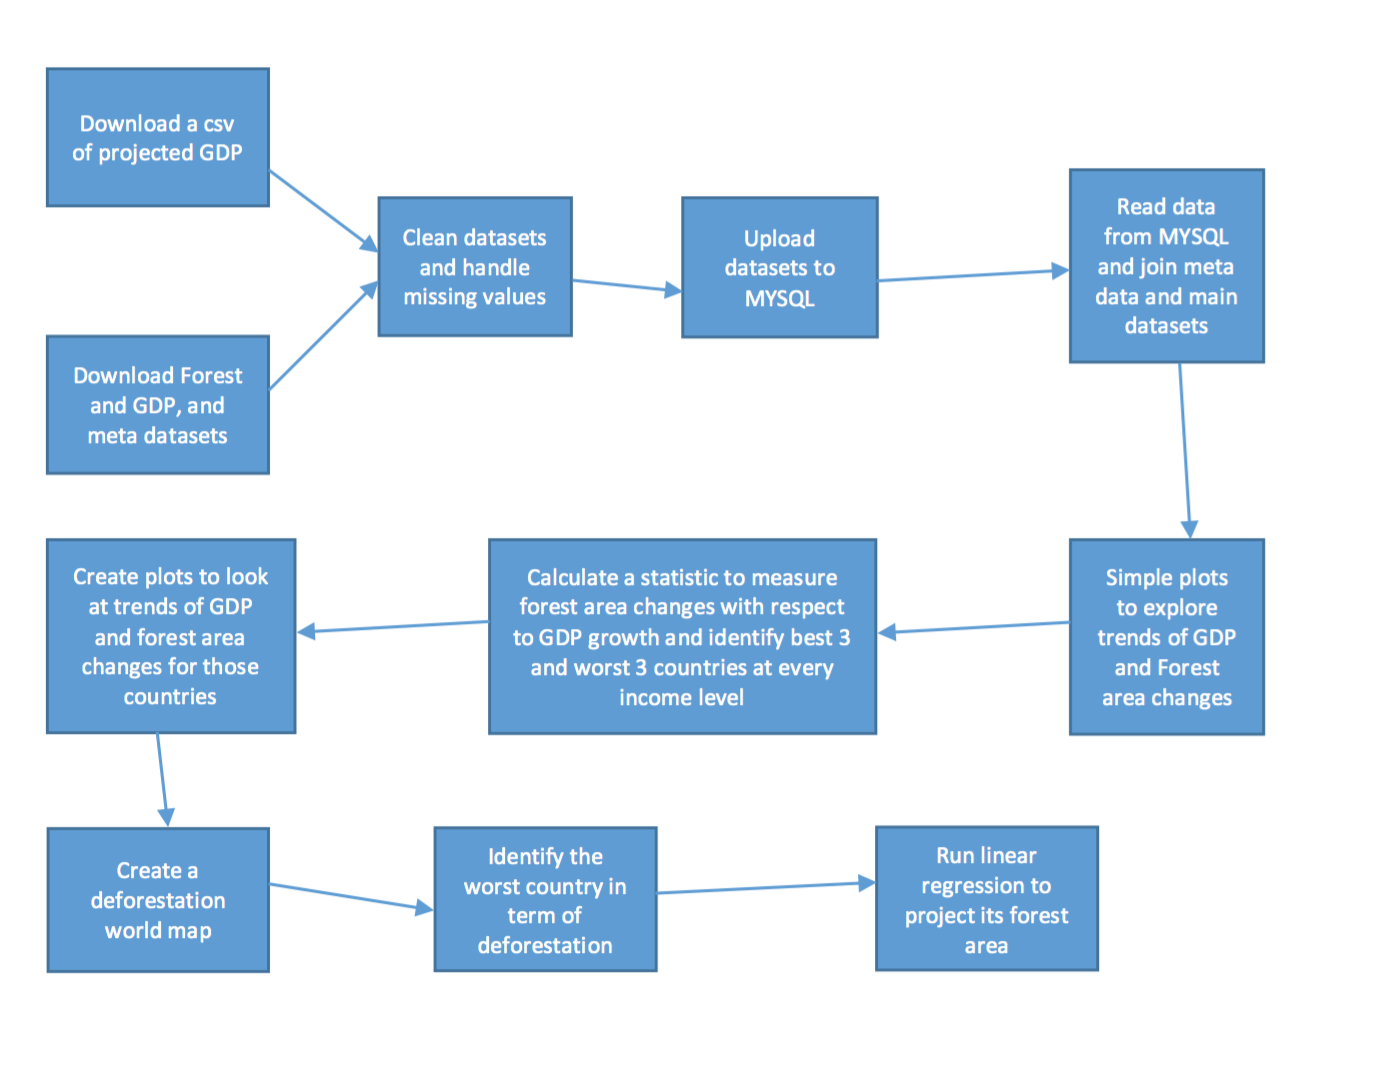
\includegraphics[scale=0.3]{workflow.png}
  \caption{The project workflow}
\end{figure}
\pagebreak
\subsection{Project structure}
The project analyzes the relationship between World Bank’s GDP and Forest Area datasets. In order to group countries by income level, additional country meta data are downloaded. After those data are cleaned, they are loaded into a MYSQL database. A SQL join query combines the datasets together. The project also develops a linear regression model to project the forest area of the worst country, in term of deforestation, for next two years using its projected GDP path.
\pagebreak
\subsection{Figures and Tables}
\begin{figure}[h]
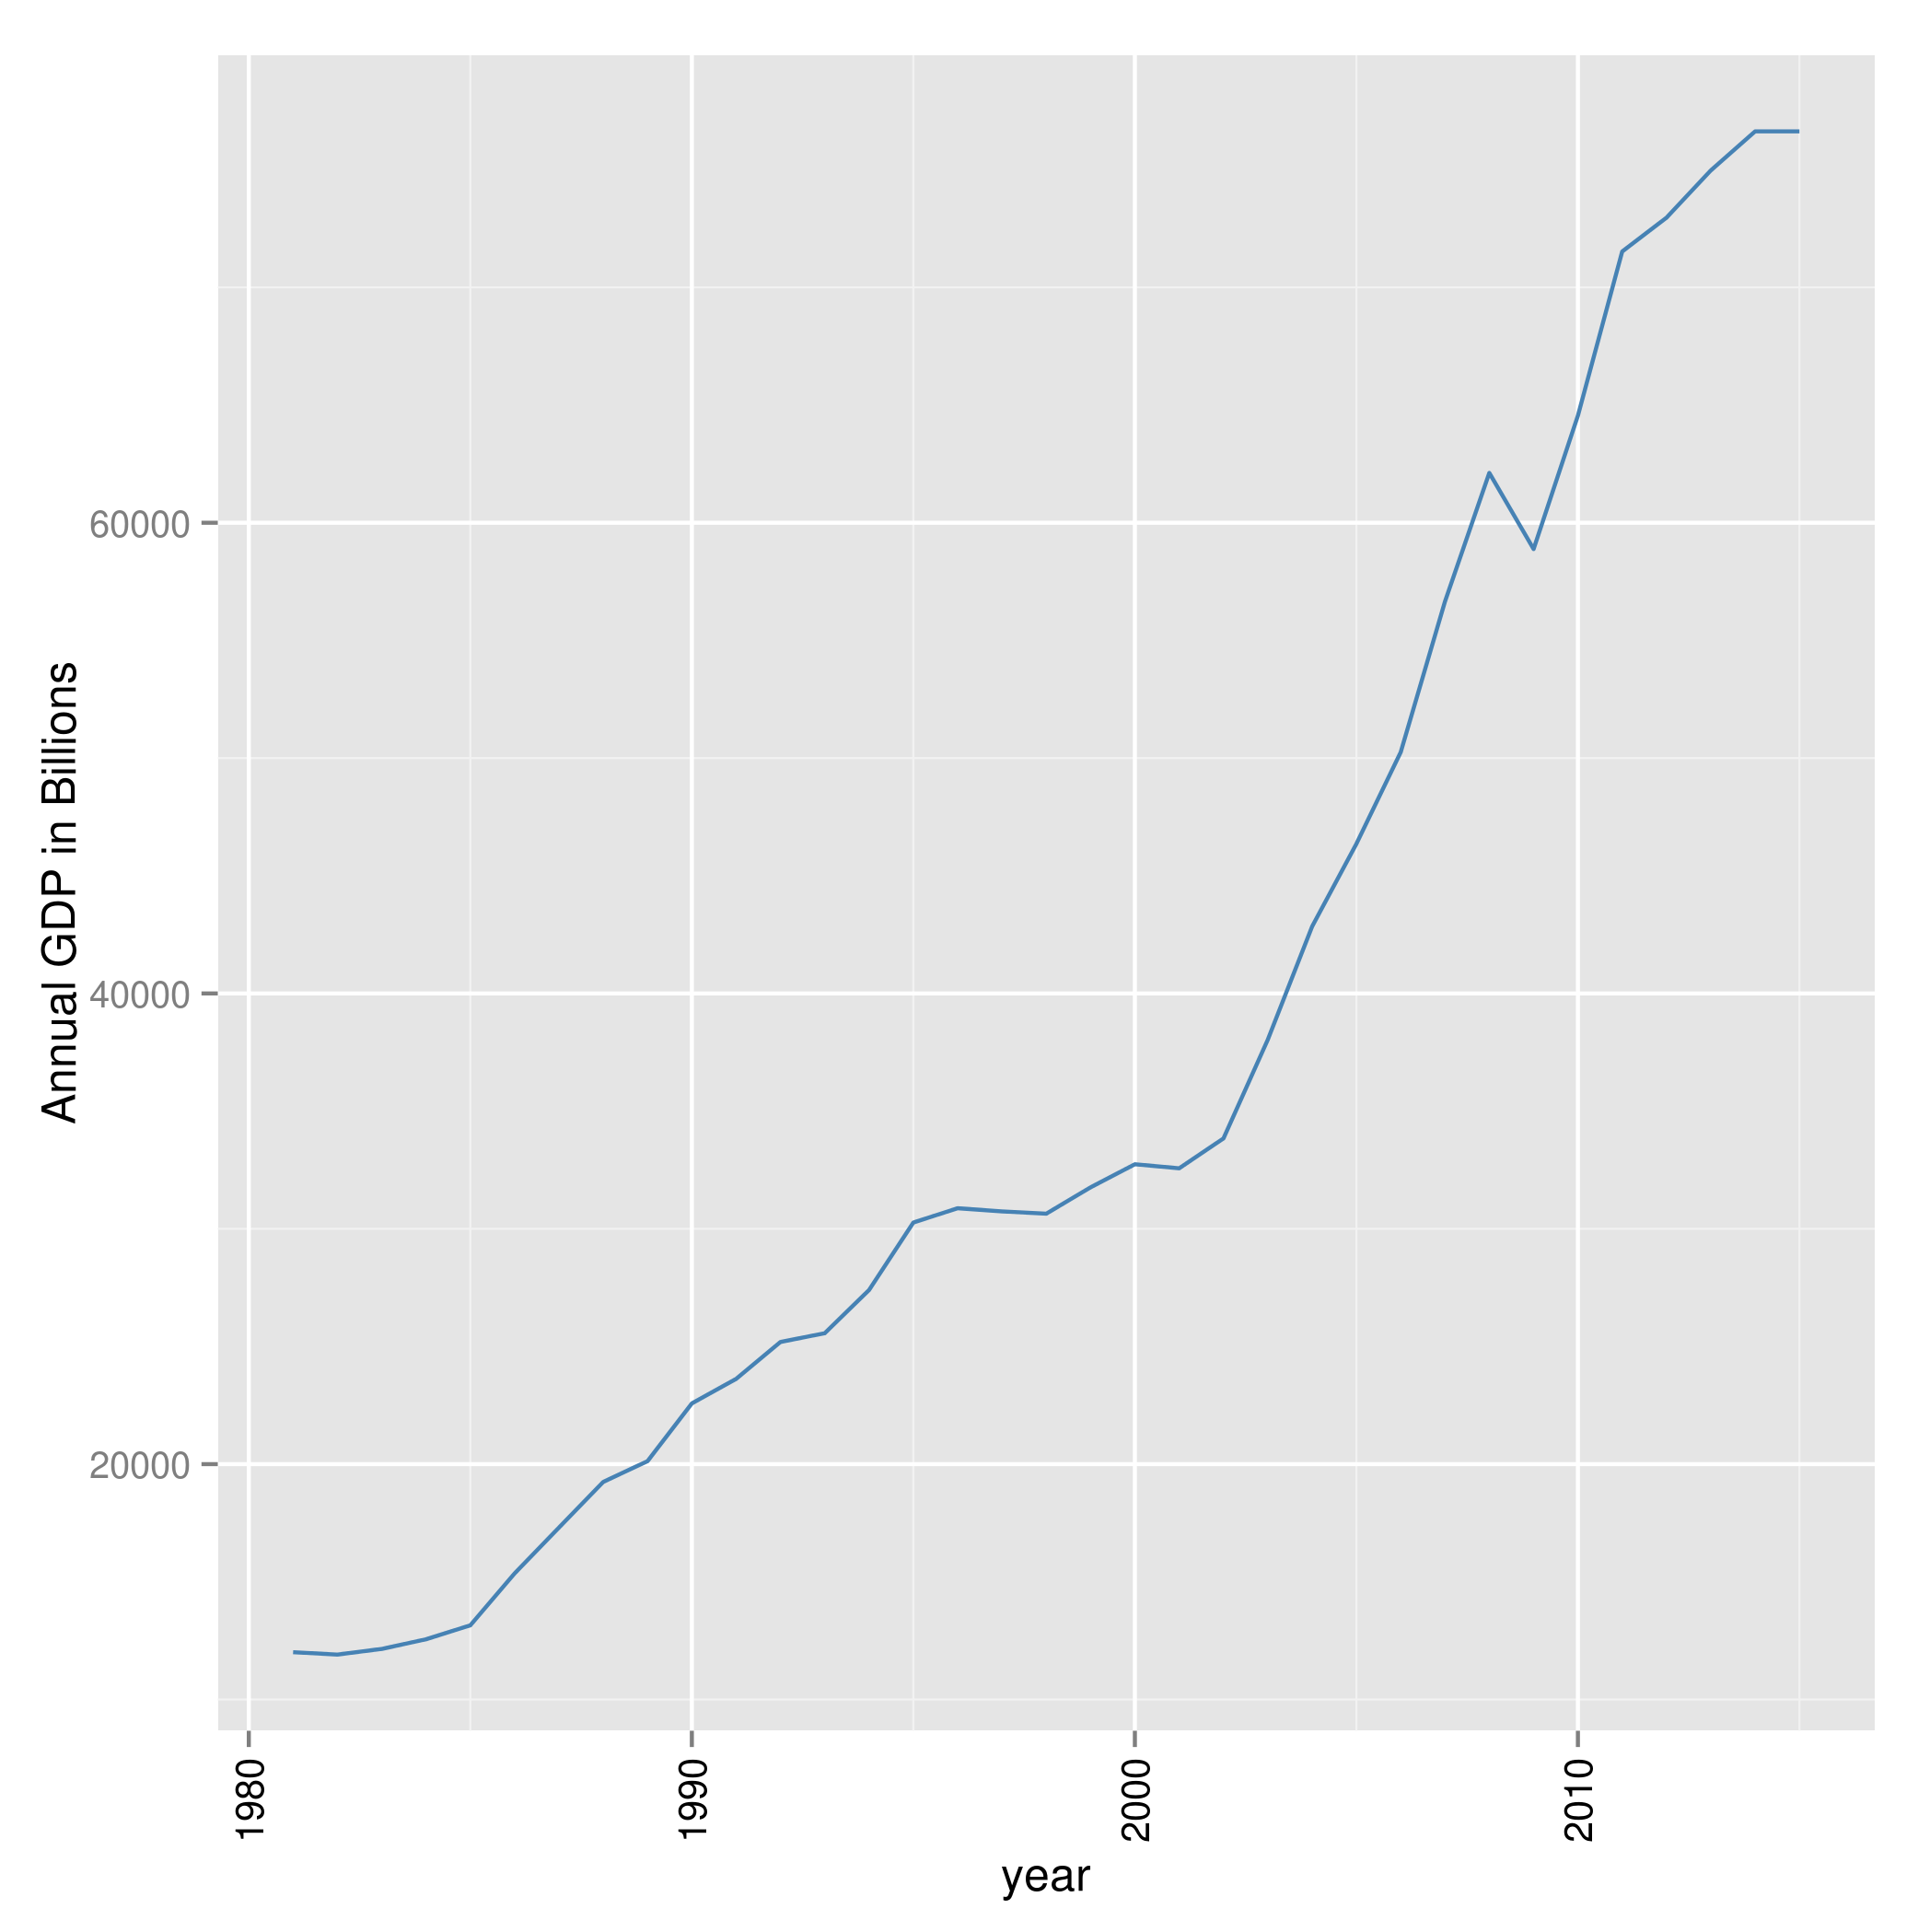
\includegraphics[scale=0.8]{gdp_total_by_year.png}
\end{figure}
\pagebreak
\begin{figure}[h]
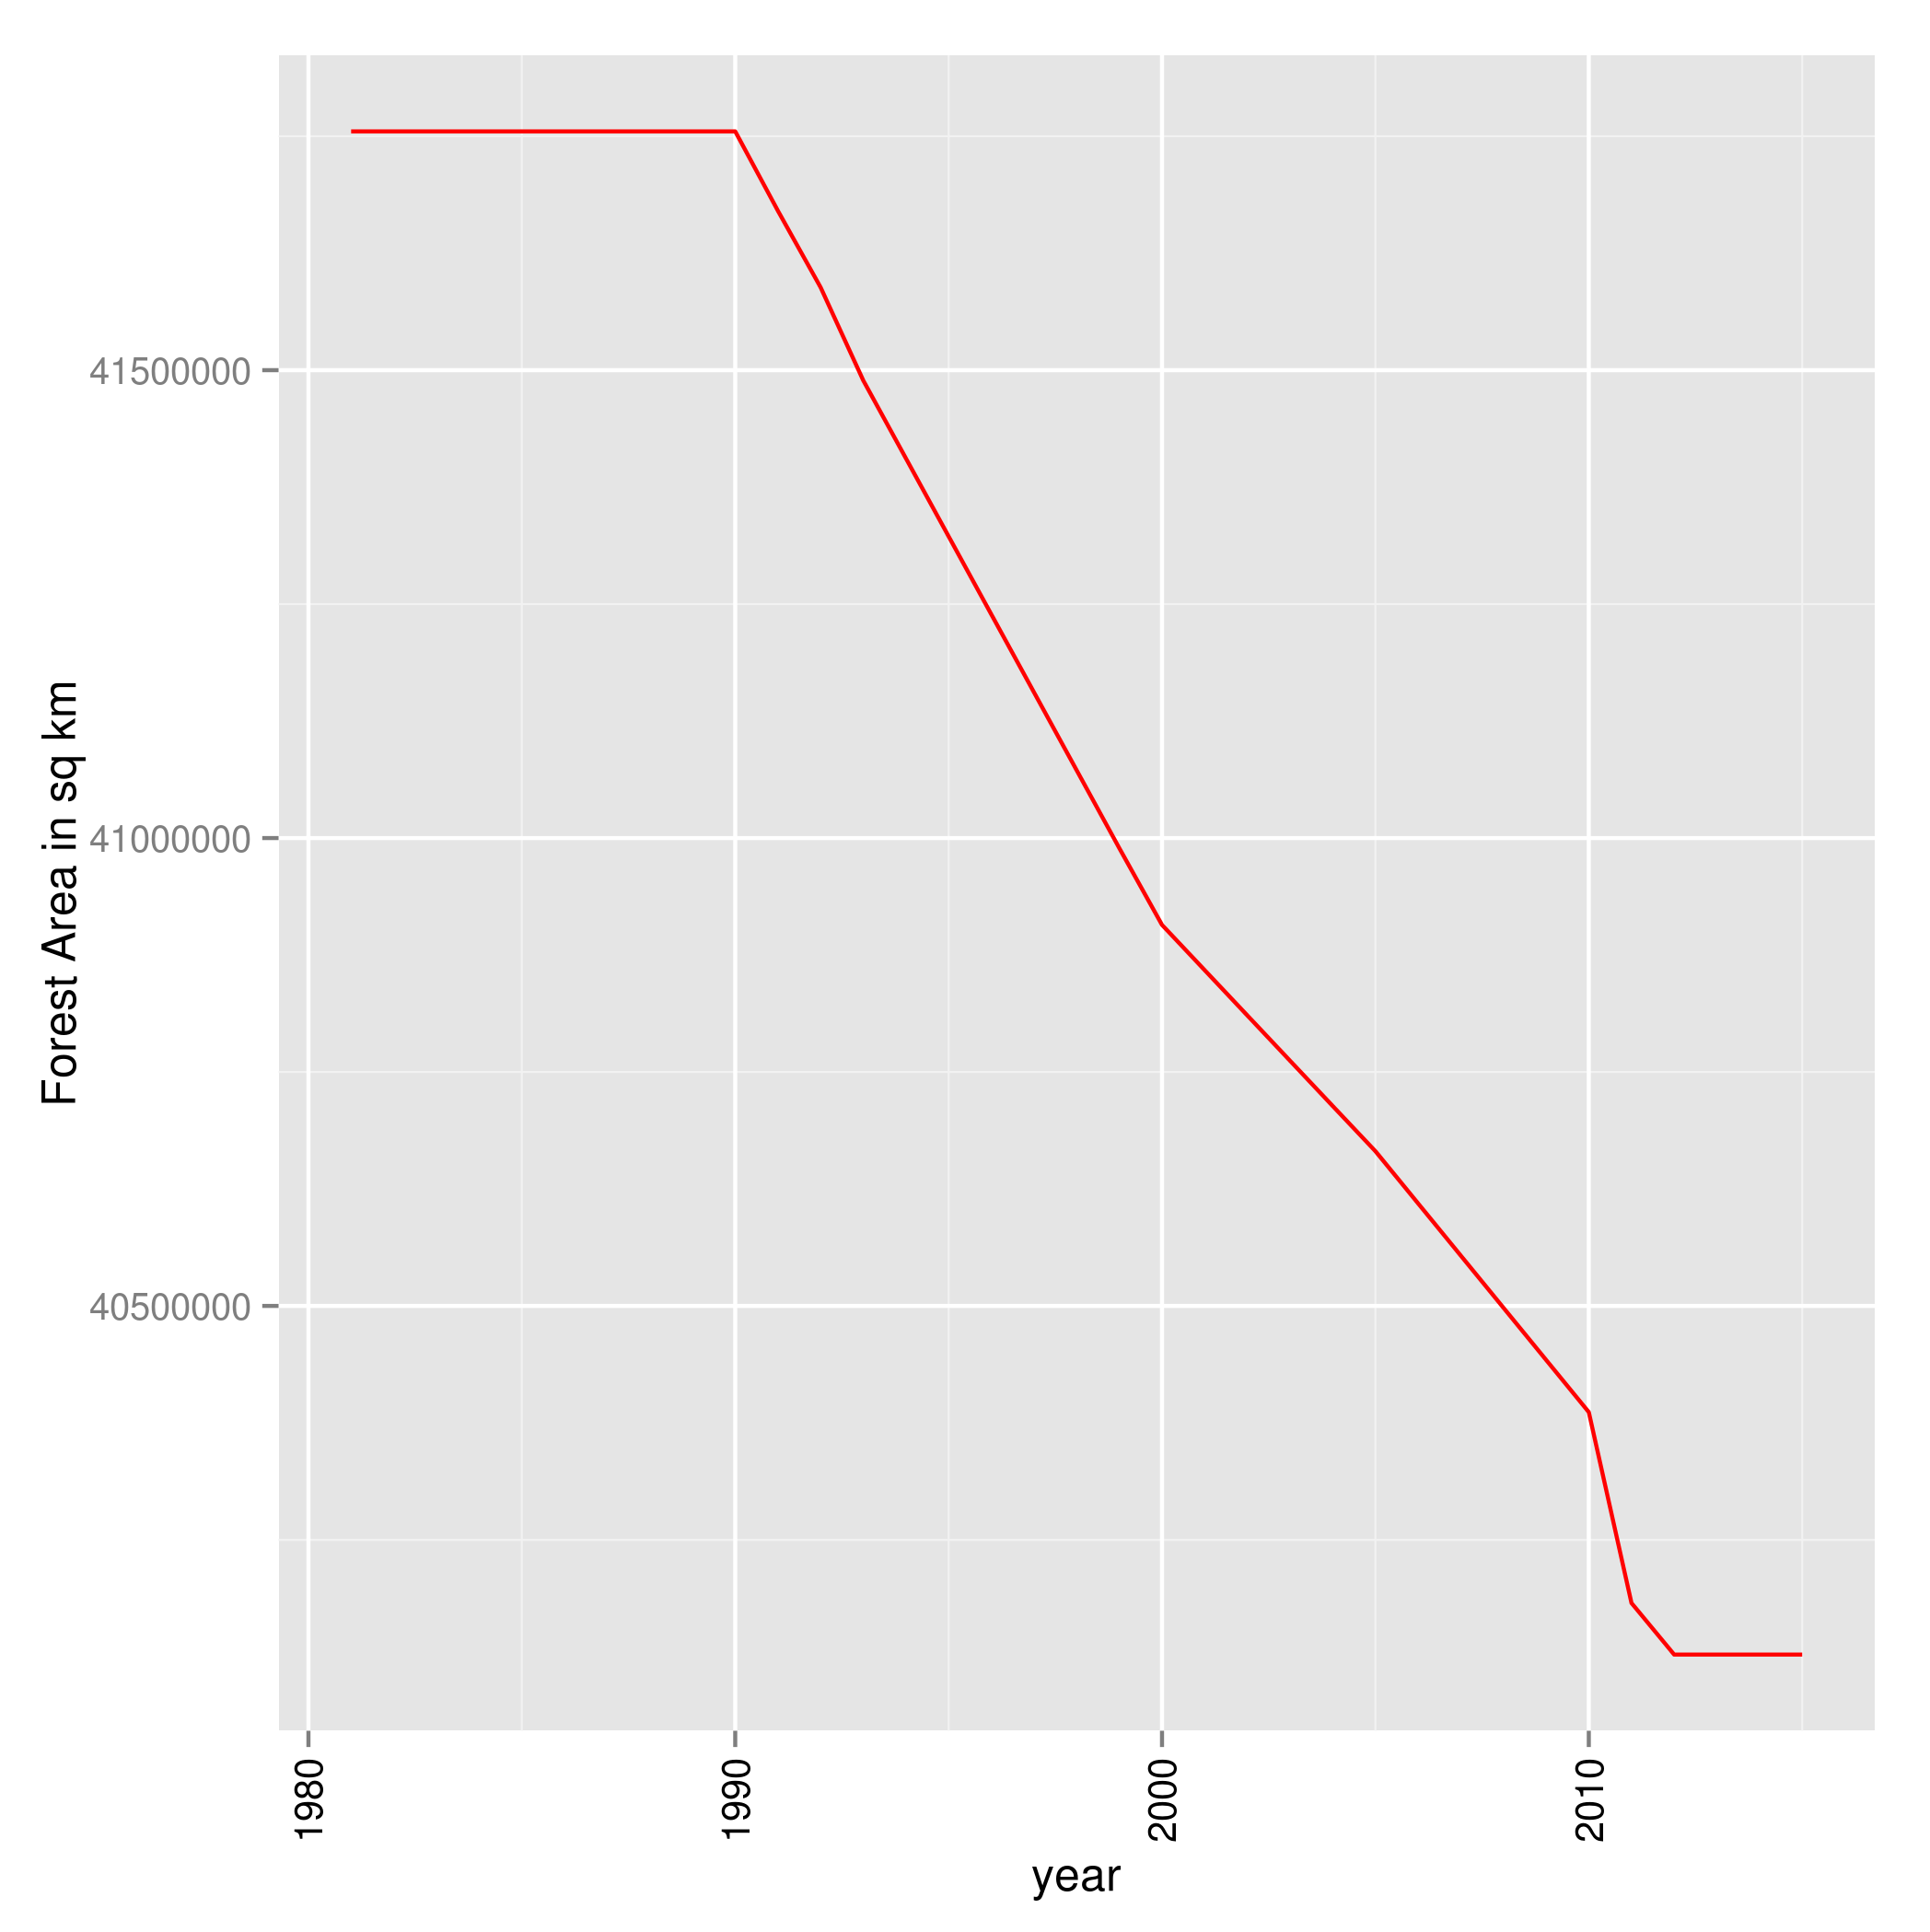
\includegraphics[scale=0.8]{forest_total_by_year.png}
\end{figure}
\pagebreak
\begin{figure}[h]
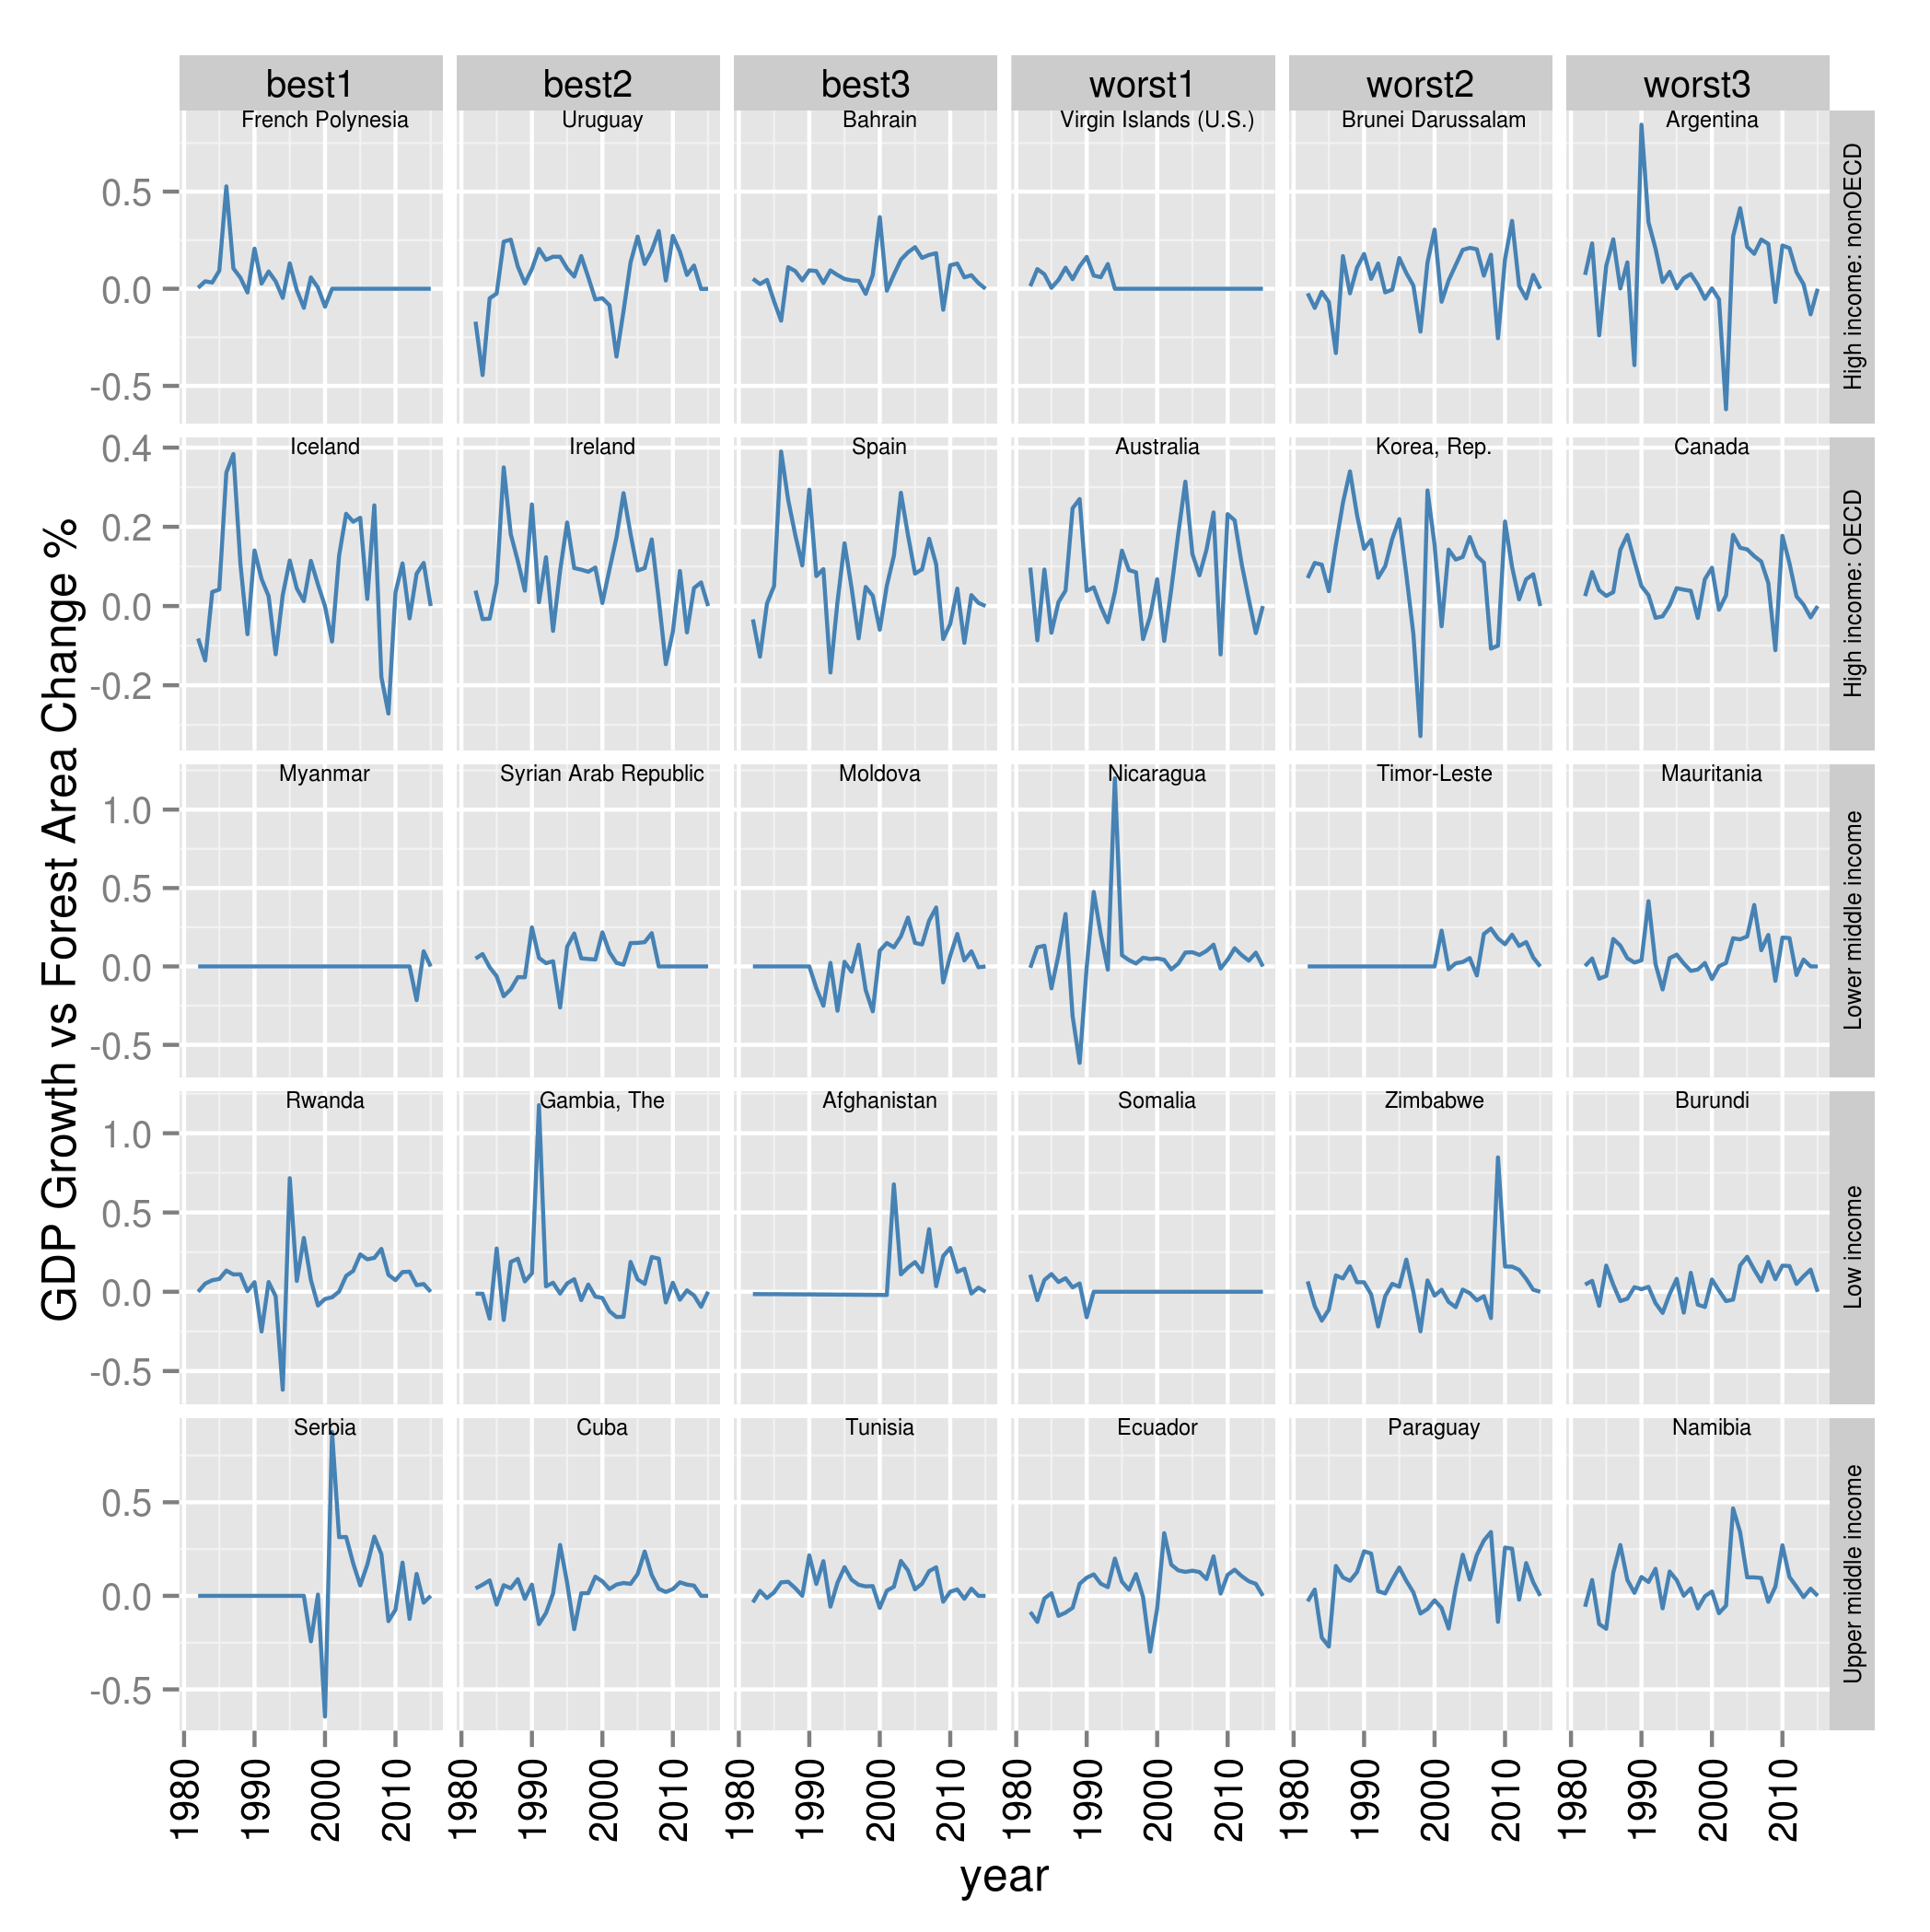
\includegraphics[scale=0.8]{gdp_by_income.png}
\end{figure}
\pagebreak
\begin{figure}[h]
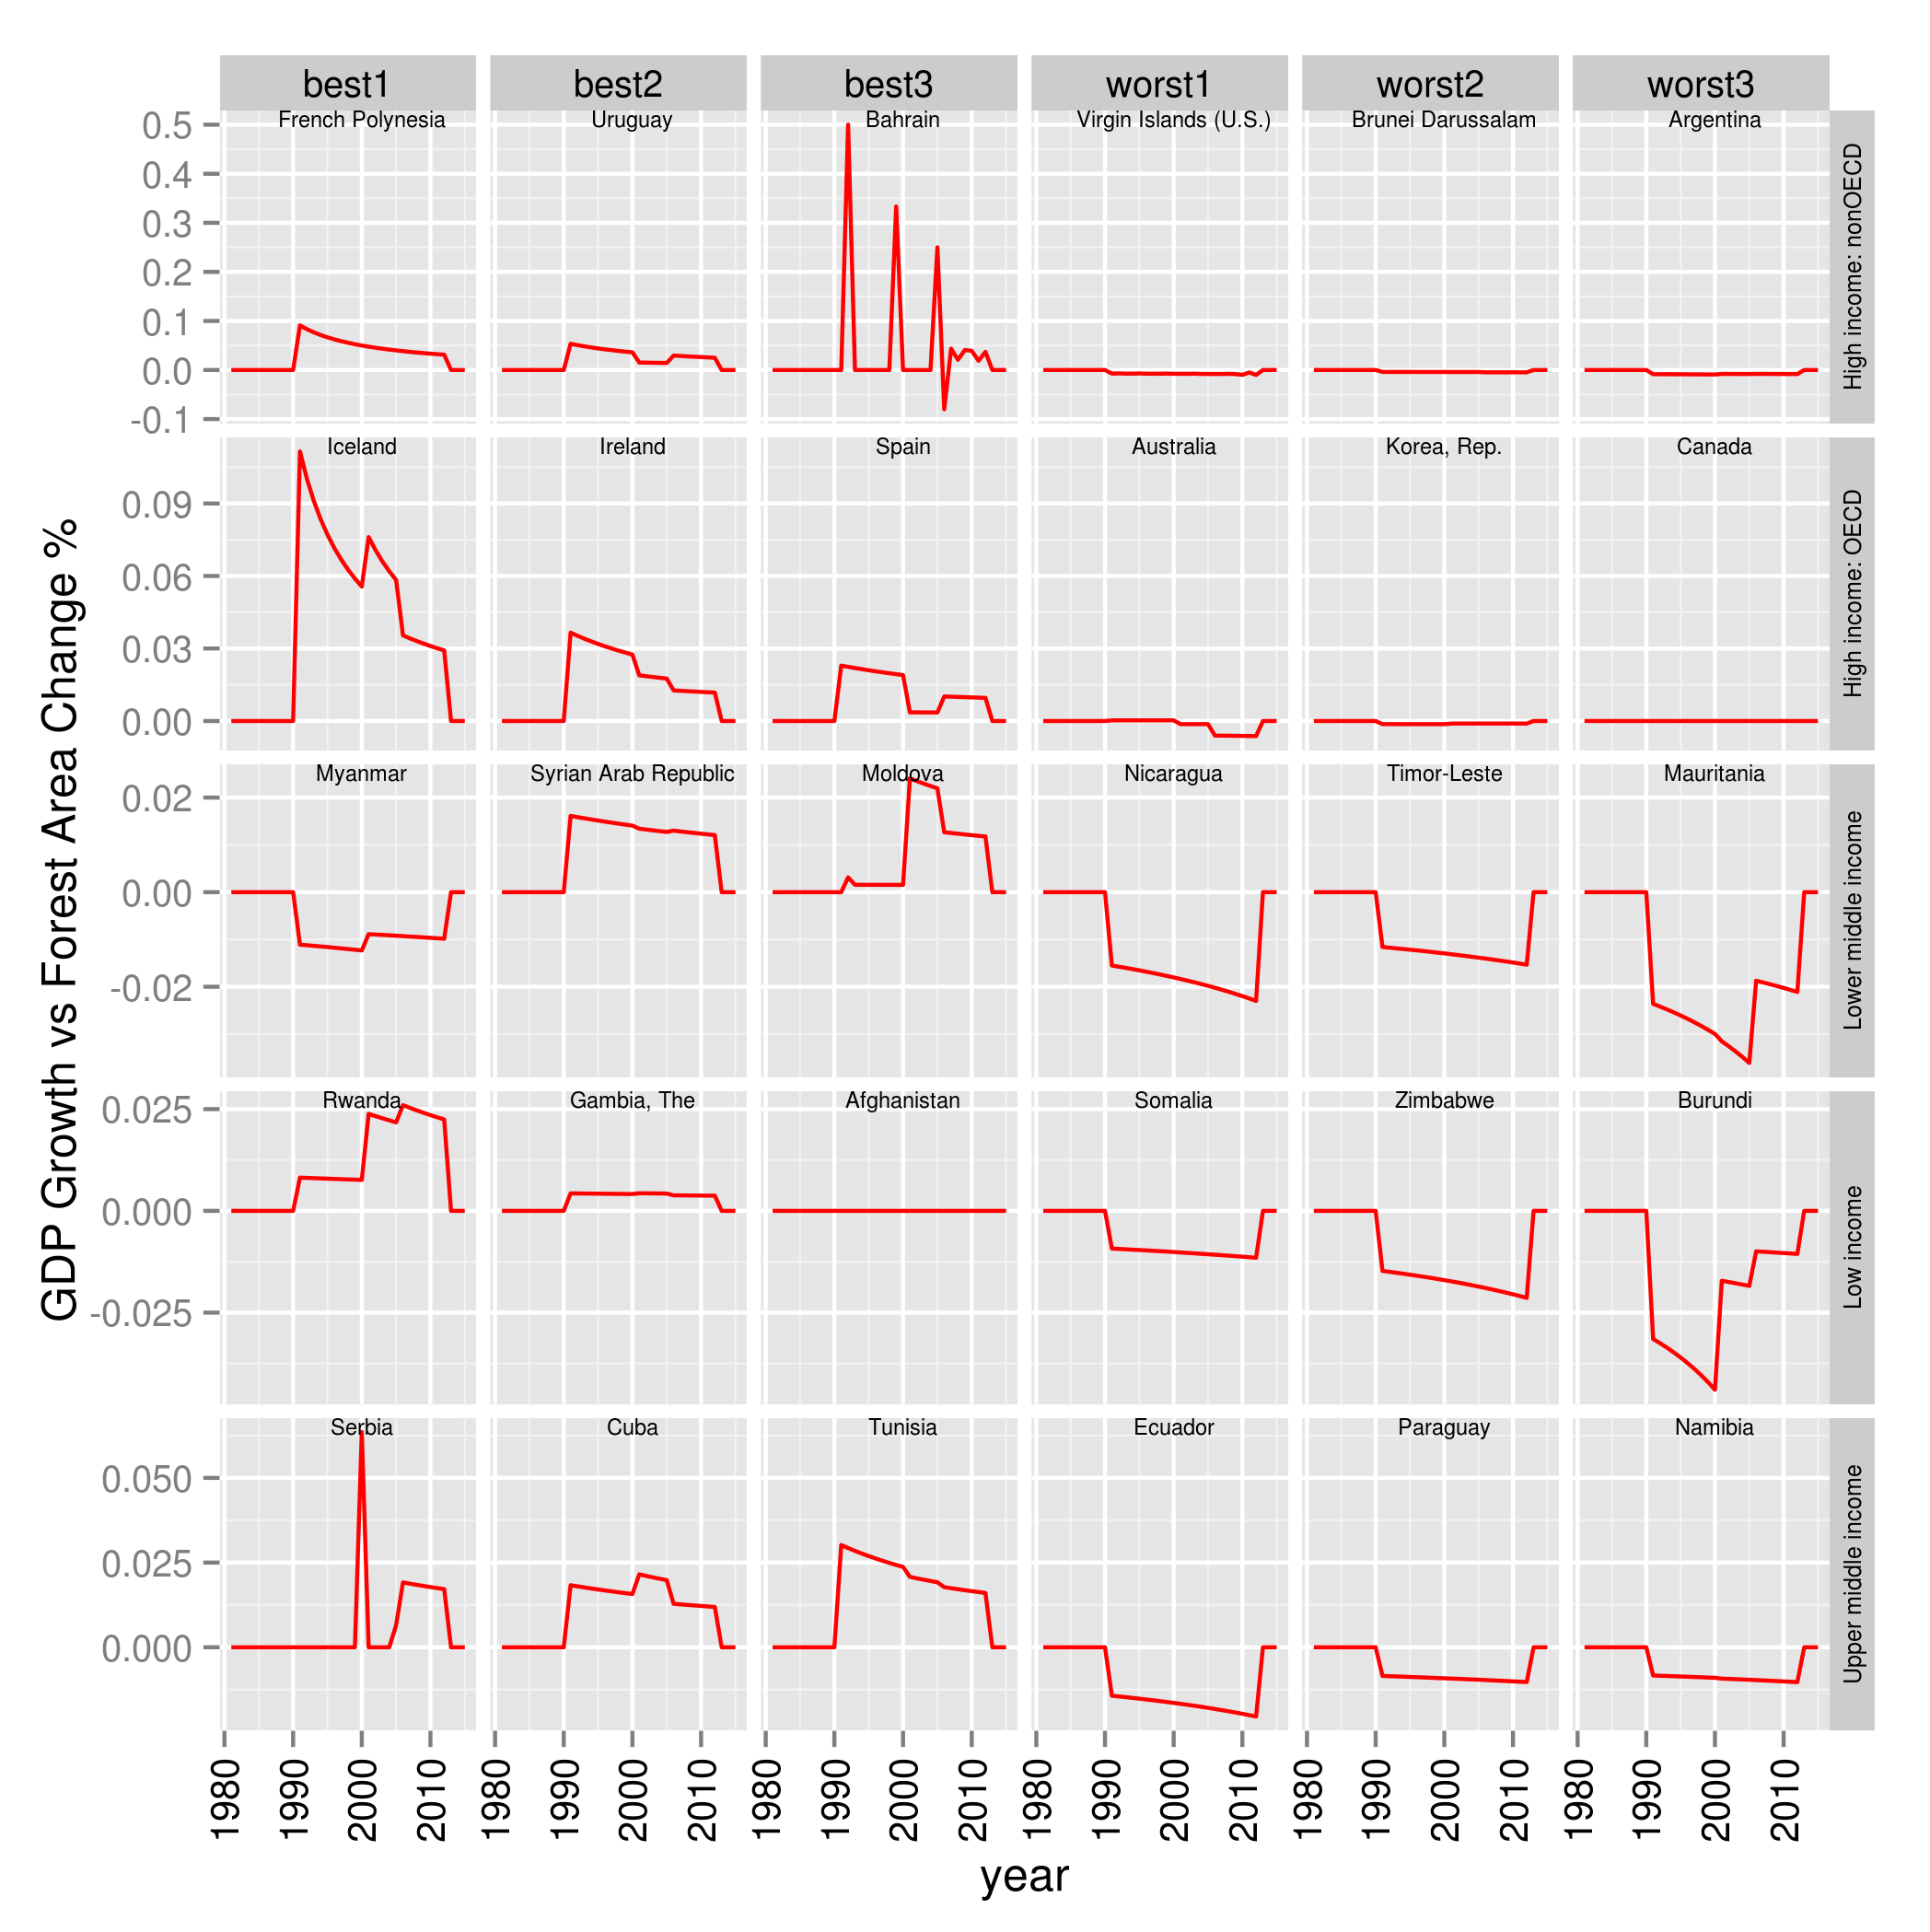
\includegraphics[scale=0.8]{forest_by_income.png}
\end{figure}
\pagebreak
\begin{figure}[h]
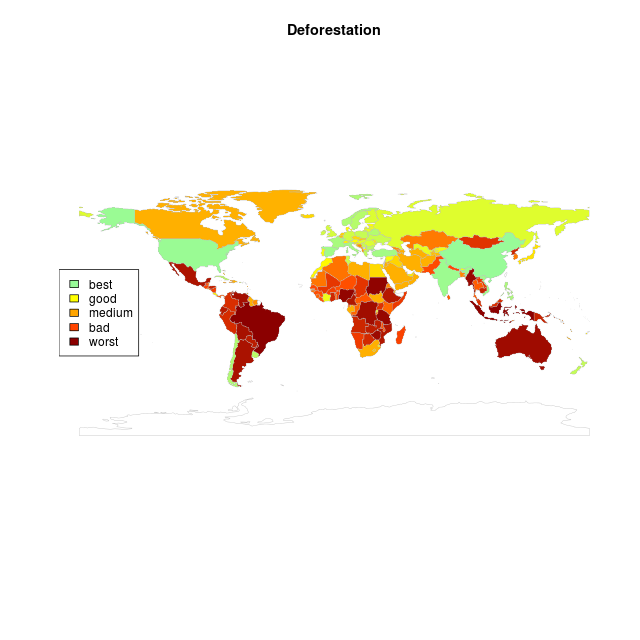
\includegraphics[scale=0.5]{wmap.png}
\end{figure}
Those figures above can be used to answer those guiding questions. The world heat map clearly shows that Latin America, Africa, and South East Asia are three worst regions in term of deforestation. 


\section{Discussion}
Although my project does not explain why some countries are doing better than other countries in protecting their forests while growing their economy, it does identify those countries at different income levels. The worst countries can draw lessons from the best countries to protect their forests while promoting economic growth. The project also demonstrates a process to create a regression model to project a nation\textquotesingle s forest area. In term of technology, the project demonstrates the possibility to utilize strength of both R and Python, the two most popular data science tools, to analyze data and built models in a reproducible manner in a ipython notebook.

\subsection{Learnings}
In this project, I learn how to utilize R to create world heat maps that allowed visualization of the country data to identify quickly which regions are worst in term of deforestation. And I aslo learn how to run R in Python using rpy2 library.

\subsection{Challenges}

One of the biggest challenges I faced is to find some datasets that are relatively clean. A lot of datasets come with missing values. So how to deal with missing values is a important problem to be solved. I use the forward filling method first to replace missing values in those time series. Then I use the backward filling method to replace missing values at the beginning of series. 



\section{Conclusion}

As we can see from plots, for the low-income countries, the African countries occupy the worst spots. But those countries can learn from the experience of Rwanda which is the best country and also an African country to protect their forests while improving standard of living of their citizens. That demonstrates the usefulness of this project. By using datasets from World Bank, we are able to investigate relationship between economic growth and forest areas changes. Hopefully, the worst countries can learn from the best countries to protect their forest areas. In term of regions, Latin America, Africa, and South East Asia clearly have lots of works to do to protect their forests.

\end{document}

